\documentclass[10pt]{article}

\usepackage{amsmath}
\usepackage{amssymb}
\usepackage{graphicx}
\usepackage{subcaption}

\begin{document}
\title{Project 1 Report}
\author{Chau Tran | Adrian Duric | Preben Castberg\\\footnotesize\texttt{cttran@uio.no} | \texttt{adriandu@uio.no} | \texttt{prebennc@uio.no}}
\date{04/09/2025}
\maketitle

\begin{abstract}
In this project we present our experiments on fine-tuning a Vision Transformer (ViT) using two approaches: full fine-tuning, where all model parameters are updated, and Low-Rank Adaptation (LoRA), where only a much smaller set of parameters is trained. We apply both methods to a classification task on the ImageWoof dataset and compare them in terms of accuracy, training time, and attention map visualizations. The key difference between the methods is that LoRA reduces the number of trainable parameters by orders of magnitude, with the goal of lowering computation and memory cost. In our results, full fine-tuning achieved higher accuracy, while LoRA gave slightly lower accuracy but showed broader attention in the visualizations. Training time was equivalent across both approaches.
\end{abstract}

\section{Introduction}
In the realm of large-scale models like Vision Transformers (ViTs), we are seeing ever increasing model sizes and more powerful embeddings, along with a growing number of use cases. A common way to adapt these models is through fine-tuning. Here we take a pre-trained model, which has learned useful embeddings on large general datasets, and adapt it into a more specific classifier trained on a smaller, task-specific dataset. \\ 

The dataset we focus on is ImageWoof, a fine-grained image classification benchmark with 10 different dog breeds. Unlike broader datasets, ImageWoof is challenging because many of the classes share similar visual features. This makes it a good testbed to study the role of fine-tuning and the attention mechanism.\\ 

In this project, our goal is to experimentally compare two fine-tuning approaches: full fine-tuning, where all model parameters are updated, and Low-Rank Adaptation (LoRA), where only a small number of additional parameters are trained. We implement both methods using the same ViT setup and measure performance, training time, and visualize the resulting attention maps.\\ 

Our main contributions are: (i) a baseline fine-tuning of ViT on ImageWoof, (ii) a LoRA implementation with the same setup, and (iii) a comparison of attention maps between the two approaches. We place particular focus on whether LoRA can achieve similar performance with fewer trainable parameters, and what differences we see in the attention visualizations. Our result are documented in detail, with the supporting metrics and visualizations, in part 4.

\section{Related Work}
In the original LoRA paper \cite{hu2021loralowrankadaptationlarge} they present us with both impressive but also necessary optimizations in fine-tuning. They fundamentally lay out the landscape of fine-tuning where huge models are expensive to fine-tune, and they show that we can bypass this limitation by restricting the trainable weights by multiple orders of magnitude. They even suggest decomposing the fine-tuned adjustments to the weights down to much lower rank matrices that approximate the patterns in the actual gradient update to the weights, they even note the use of a rank 1 matrix. Their results demonstrate a 25\% speed up in fine-tuning GPT-3 175B with LoRA compared to full fine-tuning, alongside a three-fold reduction in memory requirements.\\

The broader landscape of LoRA research has expanded significantly since its introduction. Yang et al. \cite{yang2024lowrankadaptationfoundationmodels} provide a comprehensive survey of LoRA techniques beyond their original language modeling context, examining applications across computer vision, speech recognition, and scientific discovery. They highlight that while LoRA was initially developed for LLMs, its parameter-efficient approach has found widespread adoption across diverse foundation models. The paper digs into optimizations and future directions of LoRA to ensure “scalability, and robustness” \cite{yang2024lowrankadaptationfoundationmodels}. The choice of rank is discussed as it is central to how few parameters we can get away with adjusting. They discuss both rank refinement where we vary the rank across layers or tasks adaptively, and rank augmentation, where multiple low-rank updates are combined to mimic a higher-rank 
transformation. This is intuitive to our idea of how different layers in deep neural networks are quite heterogeneous in terms of size and function. Beyond rank, they also survey methods that improve the training process itself, such as using different learning rates for the A and B matrices (LoRA+) or adjusting the scaling factor to avoid gradient collapse at higher ranks (rsLoRA).

\section{Low-Rank Adaptation}
\label{sec:lora}

Low-Rank Adaptation (LoRA) is a method that, given some pretrained weights in a neural network, indirectly continues to train the weights by freezing them, and then updating a new set of auxiliary weights which represent the change of the original weights \cite{hu2021loralowrankadaptationlarge}. Assume we have a pretrained layer of model weights $W_0 \in \mathbb{R}^{d \times k}$. LoRA indirectly updates this layer as $W_0 + \Delta W$, where $\Delta W = BA$ such that $B \in \mathbb{R}^{d \times r}$, $A \in \mathbb{R}^{r \times k}$ and $r \ll min(d, k)$ is the rank. When training the model with LoRA, $W_0$ is frozen so that only the weights in $A$ and $B$ are updated. For some input vector $x$ which would otherwise be projected as $h = W_0x$, the LoRA-based projection instead becomes:

\begin{equation}
    h = W_0x + \Delta Wx = W_0x + BAx
\end{equation}

Since both terms $W_0x$ and $BAx$ produce output vectors of the same dimensions, these vectors are summed elementwise, producing $h$.

Upon beginning training with LoRA, $A$ is initialized with randomly sampled parameters from the Gaussian distribution, while $B$ is zero-initialized, meaning $BA$ is also zero when training begins. Notice that $W_0$ contains $d \cdot k$ parameters, while $BA$ contains $d \cdot r + r \cdot k = r(d + k)$ parameters. Since $r \ll min(d, k)$, updating $\Delta W = BA$ becomes computationally cheaper to update than $W_0$, while also requiring less memory than $W_0$ to store the parameters; it can even reduce total memory usage, since no gradients need to be kept in memory for $W_0$. This makes it inexpensive to store a finetuned model with the added LoRA decomposition for deployment in production tasks.

\section{Experiments and Results}
This section details the experiments we have run, and their results.

\subsection{Finetuning ViT on ImageWoof}
\label{subsec:finetuning_vit_imagewoof}

To have a baseline performance level to which we can compare LoRA, we first finetuned a pretrained ViT \cite{dosovitskiy2021imageworth16x16words} model on the ImageWoof dataset, a subset of the ImageNet \cite{deng2009imagenet} dataset consisting of images from 10 different dog breeds. Relative to ImageNet, which contains a wide range of different image subjects, ImageWoof is more finegrained in the sense that the visual differences between different dog breeds tend to be more subtle than those between, say, a dog and a car. Differentiating between visual features that separate different dog breeds, or other similarly-looking sets of classes, is therefore typically considered a harder visual classification task than doing classification on broader-ranging sets of classes like in ImageNet.

We used the \verb|vit_tiny_patch16_224| implementation of ViT provided by the \verb|timm| \cite{rw2019timm} model library, which is pretrained on ImageNet-21k and finetuned on ImageNet2012. We replaced the classification head with one for each of the 10 ImageWoof classes. We resized each image to $224 \times 224$ pixels, and applied channelwise normalization. During training, we also randomly cropped the input images. We used a batch size of 64, and optimized using stochastic gradient descent with a learning rate of 0.001 and the cross-entropy loss function. We measured and present top-1 validation accuracy after training the model for 5 epochs on ImageWoof.

\subsubsection{Results}

We present the total training time for the standard ViT model with 5 epochs of finetuning on ImageWoof, and accuracy on the validation set. We also present curves showing the progression of training accuracy and loss.

\begin{table}[ht]
    \centering
    \begin{tabular}{c|c}
        Accuracy (\%) &  92.2 \\
        Training Time (minutes) & 18.66
    \end{tabular}
    \caption{Accuracy and training time for ViT on the ImageWoof validation set after finetuning.}
    \label{tab:placeholder}
\end{table}

\begin{figure}[ht]
    \centering
    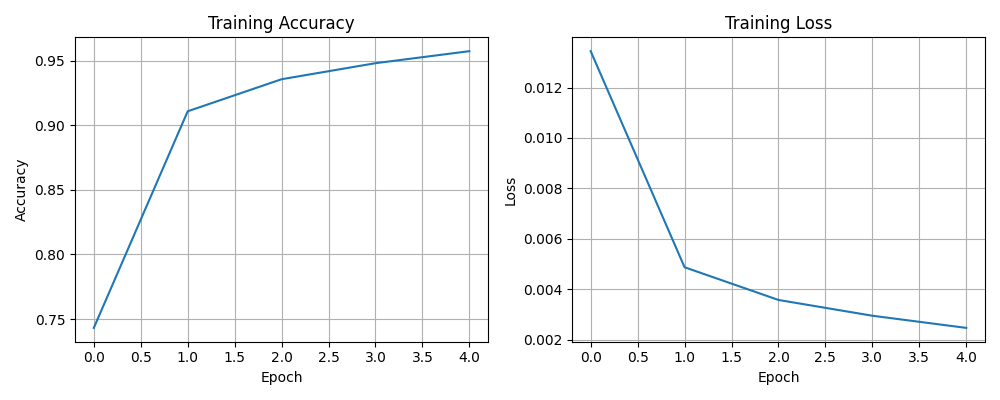
\includegraphics[width=1\linewidth]{images/training_loss_curve_vanilla.png}
    \caption{Training loss and accuracy with standard ViT on ImageWoof over 5 epochs.}
    \label{fig:placeholder}
\end{figure}

From the graphs, we observe normal behavior from the model during training. These results are compared to ViT + LoRA results in Section \ref{res_lora}.

\subsection{Finetuning ViT+LoRA on ImageWoof}

Having collected a baseline performance measurement from the standard ViT model, we then measured performance under the same circumstances when using LoRA to finetune the ViT model instead.

We implemented LoRA by freezing all layers except the classification head of the ViT. Then for the linear layers of each attention block, we initialized auxiliary linear tensors $A$ and $B$ as described in Section \ref{sec:lora}, and let $A$ and $B$ be unfreezed so their parameters can be updated. We initialized them with rank $r = 4$, one of the rank values used in the original LoRA paper \cite{hu2021loralowrankadaptationlarge}. We otherwise followed the exact same experimental configuration as detailed in Section \ref{subsec:finetuning_vit_imagewoof}.

\subsubsection{Results}
\label{res_lora}

We present the total training time for the ViT+LoRA model with 5 epochs of finetuning on ImageWoof, and accuracy on the validation set. We also present curves showing the progression of training accuracy and loss.

\begin{table}[ht]
    \centering
    \begin{tabular}{c|c}
        Accuracy (\%) &  89.0 \\
        Training Time (minutes) & 18.69
    \end{tabular}
    \caption{Accuracy and training time for ViT+LoRA on the ImageWoof validation set after finetuning.}
    \label{tab:placeholder}
\end{table}

\begin{figure}[ht]
    \centering
    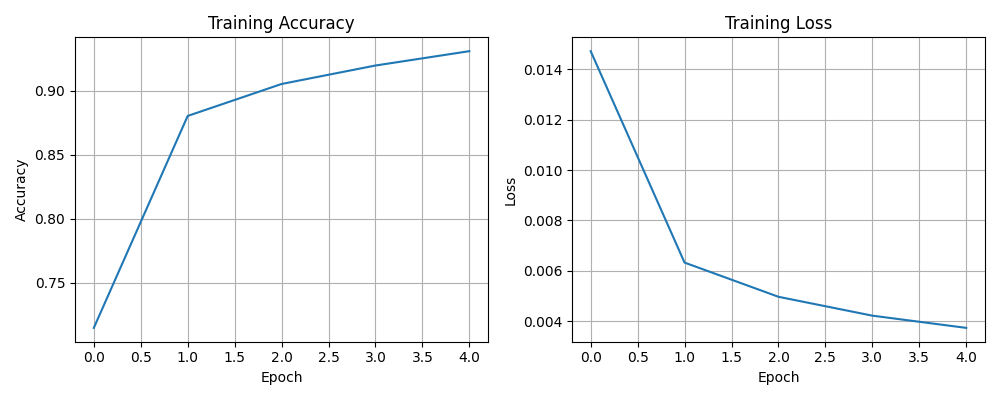
\includegraphics[width=1\linewidth]{images/training_loss_curve_LoRA.png}
    \caption{Training loss and accuracy with ViT+LoRA on ImageWoof over 5 epochs.}
    \label{fig:placeholder}
\end{figure}

We observe that the ViT+LoRA accuracy is a few percentage points lower on the ImageWoof validation set than when using the standard ViT. In terms of training time, the two models were almost exactly equal.

\subsection{Visualizing Attention Maps}

The attention mechanism in Vision Transformers (ViTs) allows the model to focus on different parts of an image when making predictions. To understand what the model ``looks at,'' we visualize these attention maps. Using functions provided in the \textit{w2\_ViT\_DINO\_DEMO} notebook, the models are slightly modified to capture the attention weights from the last attention layer, which is typically the most informative for classification tasks.

The \texttt{attention\_forward\_wrapper} function overrides the forward pass of an attention layer. While keeping the core computation logic intact, it stores the attention probabilities in \texttt{attn\_map}, allowing us to access the attention maps later without interfering with the model's normal predictions. The last attention block of each model is patched to use this wrapper, so every forward pass automatically saves the attention map for the CLS token.

To extract meaningful visualizations, the attention of the CLS token over all image patches is selected and averaged across all attention heads. This patch-level attention is reshaped into a square grid corresponding to the patch layout, upsampled to match the original image size, and normalized to a [0, 1] range. The resulting heatmap can then be visualized using helper functions. The \texttt{show\_attention\_grid} arranges multiple images and their corresponding attention maps in a grid, displaying each image alongside its attention map for side-by-side comparison. This layout follows the setup of DiNOv3 attention map figure. It allows for clear inspection of the model's focus across multiple samples, providing better insights into the inner workings of transformer models.

An example of the attention maps for both ViT and ViT+LoRA is shown in Figure~\ref{fig:attentionmaps}, highlighting differences in how the models distribute focus. In some cases, the vanilla ViT produces compact and accurate attention on the main object, while in others its attention can be diffuse or partially misplaced, sometimes highlighting background regions rather than the target. For instance, in the third image of the second row (a person holding a white dog), the vanilla ViT spreads attention over the person and surrounding area rather than concentrating on the dog. Similarly, in the last image of the first row, it attends only to fragmented parts of the dog. The ViT with LoRA often produces sharper, more object-centered attention that better covers the target. In the person-holding-dog example, LoRA correctly centers attention on the dog, and in the jumping dog case (row two, fourth column), it outlines the body more comprehensively than the vanilla ViT. However, in more complex scenes—such as an image with multiple humans playing with dogs and additional distracting items in front—the LoRA map spreads energy over the people and background, while the vanilla ViT focuses more tightly on individual dogs, though sometimes missing some of them. These examples show that LoRA tends to enhance object-focused attention, but its effect varies with image complexity and context.

\begin{figure}[htbp]
    \centering
    % Top subplot
    \begin{subfigure}[b]{1\textwidth}
        \centering
        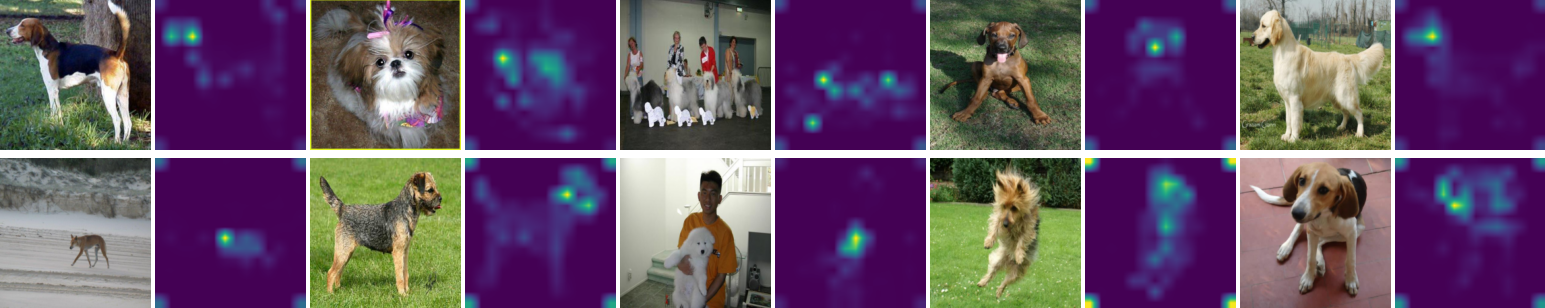
\includegraphics[width=\textwidth]{images/grid_attention_vit.png} % replace with your image
        \caption{Vanilla ViT Attention Map Sample}
        \label{fig:vit_attentionmap}
    \end{subfigure}

    \vspace{0.5cm} % optional space between subplots

    % Bottom subplot
    \begin{subfigure}[b]{1\textwidth}
        \centering
        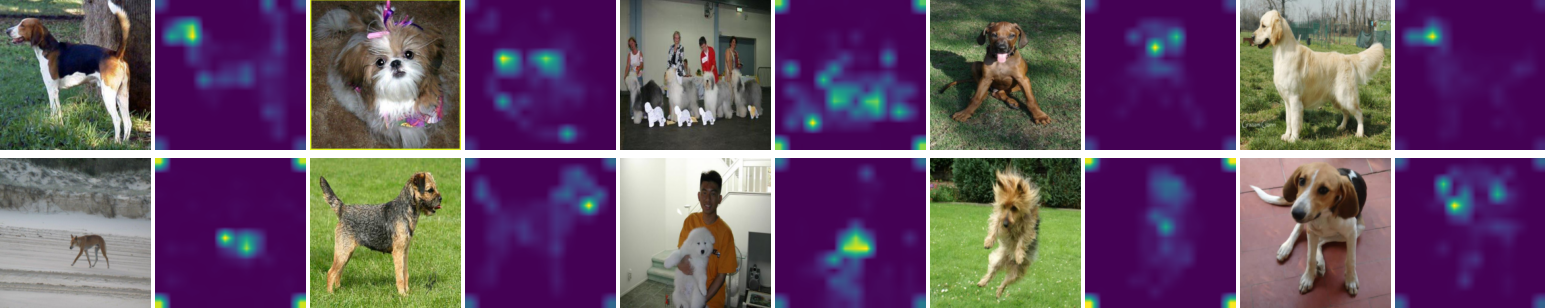
\includegraphics[width=\textwidth]{images/grid_attention_lora.png} % replace with your image
        \caption{ViT with LoRA Attention Map Sample}
        \label{fig:lora_attentionmap}
    \end{subfigure}

    \caption{An example of attention maps created from the vanilla ViT and Vit with LoRA.}
    \label{fig:attentionmaps}
\end{figure}

\section{Discussion}
ViT with LoRA introduces low-rank adapters in place of fully fine-tuning all parameters of the Vision Transformer. This approach is expected to reduce the number of trainable parameters, thereby lowering memory requirements and potentially speeding up training. However, in our experiments, we did not observe a noticeable difference in training time between the vanilla ViT and ViT+LoRA. One possible explanation is the relatively small size of the ViT-Small model used in this study. Since the full model already contains a modest number of parameters, freezing them does not bring a substantial efficiency gain, and the additional LoRA matrices (A and B) may offset the expected savings. For larger backbone models (e.g., ViT-Base or ViT-Large), the trade-off would likely become more apparent.

Although the attention maps show that ViT+LoRA is more object-centered and produces sharper, semantically meaningful focus on the target objects, the vanilla ViT achieves higher classification accuracy. A hypothesis reason can be the capacity trade-off. It means by constraining parameter updates to a low-rank subspace, LoRA reduces representational flexibility, which can slightly hurt performance in cases where full fine-tuning can exploit all available capacity. LoRA is still very useful in cases where saving memory and training time is more important than getting the very best accuracy. For example, it works well on smaller devices with limited resources, or in fields like medical imaging where we want the model’s attention to be clear and trustworthy. Another advantage is that we can train small LoRA adapters for different tasks (like one for classifying medical scans and another for satellite images) without retraining the whole model each time.

\section{Conclusion}
In this study, we set out to compare full fine-tuning and LoRA-based fine-tuning of Vision Transformers on the ImageWoof benchmark. While LoRA was expected to reduce the number of trainable parameters and ease the training burden, our experiments with ViT-Small showed little difference in training time compared to the vanilla setup. Moreover, we observed that the vanilla ViT achieved higher classification accuracy, even though LoRA produced more object-centered and interpretable attention maps. This suggests that on smaller backbones, the parameter savings of LoRA are offset by a loss in representational flexibility. 

Nevertheless, LoRA remains attractive in scenarios where efficiency, modular adaptation, or interpretability are valued over raw accuracy—for instance, in resource-constrained environments or safety-critical applications like medical imaging. Future work should extend this comparison to larger ViT models and more diverse datasets, where LoRA’s advantages may become more pronounced.

\section{Group Contributions}

For the programming, Adrian wrote the code for the LoRA wrapper, freezing and unfreezing relevant parts of the models and the training and testing of the models. Preben wrote the code for conducting the first two experiments and obtaining result metrics that were presented in this report. Chau wrote the code for visualizing the attention maps with and without LoRA, the third experiment.

For the report, Preben wrote the abstract, introduction and related work parts. Adrian wrote the methods part, as well as the experiment and results and conclusion parts regarding the first two experiments. Chau wrote the equivalent parts for the third experiment, as well as the discussion part.

\bibliographystyle{IEEEtran}
\bibliography{report}

\end{document}